\documentclass[12pt, a4paper, twoside, UKenglish]{article}
\usepackage[utf8]{inputenc}
\usepackage[T1]{fontenc,url}
\urlstyle{sf}
\usepackage{babel,textcomp,csquotes,graphicx}
\usepackage[nospace]{varioref}
\usepackage[backend=biber,style=numeric-comp]{biblatex}
\usepackage{amsfonts}
\usepackage[margin=2cm,nohead]{geometry}
\graphicspath{ {images/} }


\title{Essay}
\author{Espen Lønes}
\date{\today}

\bibliography{refs.bib}

\begin{document}

\maketitle

\tableofcontents{}
\listoffigures{}
\listoftables{}

\section{Introduction}
Ultrasound imaging is frequently used in the medical sector. The  major advantage over other common types of imaging (e.g. X-ray, CT, MRI) is that ultrasound provides interactive real-time imaging.
This combined with its relatively low cost has cemented it its place in the medical field.\\
\ \\
The real-time aspect of ultrasound imaging also means it is has limited processing time before the image has to be displayed. This limits the amount of prepossessing one can do to the images. The type of preprocessing we will discuss is adaptive beamforming. Many [Most/All] of the adaptive beam-formers take to long to be used in real-time ultrasound. One way of avoiding this heavy computation is by using a neural-network to estimate the true calculations. This approach has been used by \cite{Adaptive-Deep-Learning, Kjenstad} with varying results.\\
\ \\

\section{Cite test}
\cite{Krim-Viberg, Models-to-Deep, Rindal, DNN-beamforming, Kjenstad, NN-eigen, Simons, Adaptive-Deep-Learning}\\

\section{Background}

\subsection{Ultrasound}
Ultrasound imaging works by having a transducer usually consisting of an array of transmit/receive elements. Each element will produce a spherical wave-front. Array transducers can apply individual delays to each element s.t. the interference pattern between the spherical waves form a steered narrow beam in a desired direction. (see beamforming)\\
\ \\

The imaging is based on the pulse echo principle. This is done by recording the reflections of the emitted sound beam we just discussed. As the sound propagates trough the medium (e.g. the human body) different structures and materials will reflect the sound different amounts. These changes in reflection amplitude over time is what we receive/record on the elements of the transducer. If we know the sound speed in our medium we can translate our time data to distance giving us the ability to make images with real distance units.\\
\ \\

\subsection{Who uses it}
Medical.\\
Manipulation and characterization of particles (ultrasound attenuation spectroscopy, electroacoustic phenomena).\\
Wireless communication (underwater, cross-device tracking).\\
Elliptic labs.\\ 


\subsection{Beamforming}

\subsubsection{DAS}
Delay and Sum or DAS, is the most basic / standard form of beamforming.
The technique is similar to the focusing of the beam discussed in the ultrasound section.
First i will use the example of receive beamforming but for transmit beamforming we do the same in reverse order.\\
An illustration of receive DAS is seen in Figure~\vref{DAS}.\\
DAS uses the fact that since the elements (M) will have slightly different distances to the source if the sound (S). The received signals will be out of phase. By applying different time delays to each element, corresponding to the relative positions to each-other and the source. Signals from sources in a chosen direction can be aligned s.t. when adding them together they constructively sum (as seen in a)). As we see in b) sources not in the correct place given by our choice of delays will not constructively sum. Resulting in off axis signals to be attenuated compared to on axis.\\    
\ \\
As mentioned in ultrasound transmit beamforming one delays transmitting signals on each element instead. The delays are chosen s.t. the waves arrive at a focal point simultaneously.
In this direction high pressure builds and reaches its maximum at the focal point. This region has the name main lobe. To the sides of the main lobe we also get beams of pressure but these have less energy as they are partially out of phase, these are called the side lobes. The relative difference in energy between the main and side lobes as well as main lobe with are the main factors for image quality.\\   
\ \\

\begin{figure}[!htb]
	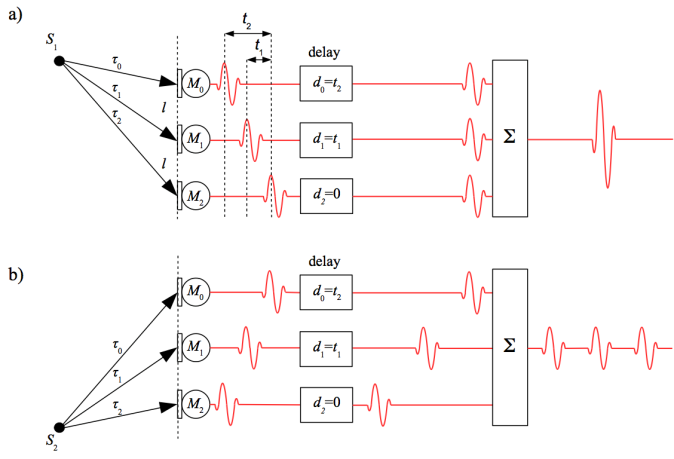
\includegraphics[scale=0.6]{DAS.png}
	\caption{a) $S_1$ from target position. b) $S_2$ off target signal / noise\label{DAS}}
\end{figure}

\subsection{Adaptive beamforming}
One of the ways to further manipulate the data is to apply weighting or apodization to the individual element signals. One way to do this is to use a predefined set/shape of weights. e.g. hamming, hanning, blackman. (\textbf{Find reference}). Another way is to use characteristics of the signal itself to define the apodization. This is what is called adaptive beamforming.\\
Examples of these are Capons's or Minimum variance, Music and other eigenvector methods.\\
These methods can often greatly improve image quality (\textbf{Reference}), but it comes at the cost of increased computation. As the methods usually require either inverting a large matrix or calculating a set eigenvalue, eigenvector pairs.

\subsubsection{Capon's / MV beamformer}
\cite{Krim-Viberg}
\subsubsection{Eigenvalue / Eigenvector methods}
\cite{Krim-Viberg}
\subsection{Coherence}

\subsection{ML}
	
\subsubsection{Supervised learning}
Supervised learning is the subclass of machine learning used by \cite{Adaptive-Deep-Learning, Kjenstad}. It consists of having a set of data with given labels/solutions telling the model what the solution when the corresponding data is given as input. Our goal is to make the model learn how to respond to new data and give us the correct label or solution. In our example the data would be the recorded ultrasound data. Solutions would be pre computed apodization weights. And our goal is for the model to learn to make the correct weights for new data.\\
\ \\

\subsubsection{NNs and DNNs}
The type of model use for supervised learning by  \cite{Adaptive-Deep-Learning, Kjenstad} are Neural-Networks or NNs. Specificity Deep NNs or DNNs. A non-deep and a DNN are illustrated in Figure~\vref{NN/DNN}. A DNN consist of a input layer, multiple hidden layers and one output layer. All layers have a sett amount of nodes, for us the input corresponds to the shape of our data, the hidden layer sizes can be chosen, the output will be the apodization weights. Both \cite{Adaptive-Deep-Learning, Kjenstad} used fully connected networks where every node from one layer is connected to every node in the next layer.
\\
\ \\

\begin{figure}[!htb]
	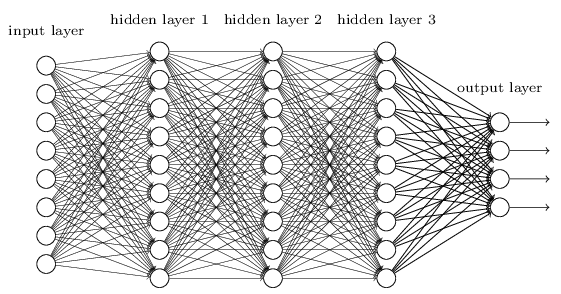
\includegraphics[scale=0.6]{DNN.png}
	\caption{Structure of a NN (left) and a DNN (right)\label{NN/DNN}}
\end{figure}

\subsubsection{Variational networks}
??\\
\ \\

\section{Discussion}
??\\
\ \\

\printbibliography

\end{document}